60. \begin{figure}[ht!]
\center{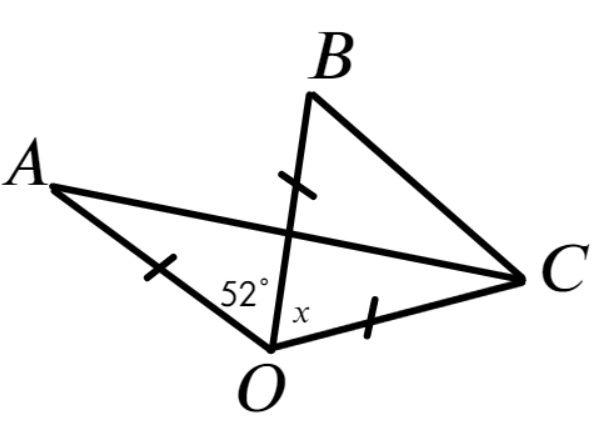
\includegraphics[scale=0.35]{g60.png}}
\end{figure}\\
Обозначим $\angle BOC=x.$ Треугольник $AOC$ равнобедренный с углом при вершине $x+52^\circ,$ поэтому $\angle ACO=(180^\circ-52^\circ-x):2=64^\circ-\frac{1}{2}x.$ Треугольник $BOC$ равнобедренный с углом при вершине $x,$ поэтому $\angle OCB=(180^\circ-x):2=90^\circ-\frac{1}{2}x.$ Таким образом, $\angle ACB=90^\circ-\frac{1}{2}x-(64^\circ-\frac{1}{2}x)=26^\circ.$\\
